\documentclass[aspectratio=169]{beamer}

\mode<presentation>
{
  \usetheme{default}
  \usecolortheme{default}
  \usefonttheme{default}
  \setbeamertemplate{navigation symbols}{}
  \setbeamertemplate{caption}[numbered]
  \setbeamertemplate{footline}[frame number]  % or "page number"
  \setbeamercolor{frametitle}{fg=white}
  \setbeamercolor{footline}{fg=black}
} 

\usepackage[english]{babel}
\usepackage[utf8x]{inputenc}
\usepackage{tikz}
\usepackage{courier}
\usepackage{array}
\usepackage{bold-extra}
\usepackage{minted}
\usepackage[thicklines]{cancel}

\xdefinecolor{dianablue}{rgb}{0.18,0.24,0.31}
\xdefinecolor{darkblue}{rgb}{0.1,0.1,0.7}
\xdefinecolor{darkgreen}{rgb}{0,0.5,0}
\xdefinecolor{darkgrey}{rgb}{0.35,0.35,0.35}
\xdefinecolor{darkorange}{rgb}{0.8,0.5,0}
\xdefinecolor{darkred}{rgb}{0.7,0,0}
\definecolor{darkgreen}{rgb}{0,0.6,0}
\definecolor{mauve}{rgb}{0.58,0,0.82}

\title[2017-10-25-aps-nuclear]{Bridging the Particle Physics and Big Data Worlds}
\author{Jim Pivarski}
\institute{Princeton University -- DIANA-HEP}
\date{October 25, 2017}

\begin{document}

\logo{\pgfputat{\pgfxy(0.11, 7.4)}{\pgfbox[right,base]{\tikz{\filldraw[fill=dianablue, draw=none] (0 cm, 0 cm) rectangle (50 cm, 1 cm);}\mbox{\hspace{-8 cm}
\includegraphics[height=1 cm]{princeton-logo-long.png}
\includegraphics[height=1 cm]{diana-hep-logo-long.png}}}}}

\begin{frame}
  \titlepage
\end{frame}

\logo{\pgfputat{\pgfxy(0.11, 7.4)}{\pgfbox[right,base]{\tikz{\filldraw[fill=dianablue, draw=none] (0 cm, 0 cm) rectangle (50 cm, 1 cm);}\mbox{\hspace{-8 cm}
\includegraphics[height=1 cm]{princeton-logo.png}
\includegraphics[height=1 cm]{diana-hep-logo.png}}}}}

% Uncomment these lines for an automatically generated outline.
%\begin{frame}{Outline}
%  \tableofcontents
%\end{frame}

%%%%%%%%%%%%%%%%%%%%%%%%%%%%%%%%%%%%%%%%%%%%%%%%%%%%%%%

%%%% START

%% \begin{frame}{The original Big Data}
%% \vspace{0.5 cm}

%% \large For decades, physicists' computing needs were unique:

%% \vspace{0.1 cm}
%% \begin{itemize}
%% \item big datasets \hfill \begin{minipage}{0.7\linewidth}(too large for one computer: a moving definition!),\end{minipage}
%% \item complex structure \hfill \begin{minipage}{0.7\linewidth}(nested data, web of relationships within each event),\end{minipage}
%% \item has to be reduced \hfill \begin{minipage}{0.7\linewidth}(aggregated, by histogramming, usually)\end{minipage}
%% \item to be modeled \hfill \begin{minipage}{0.7\linewidth}(fitting to extract physics results).\end{minipage}
%% \end{itemize}

%% \vspace{0.5 cm}
%% \uncover<2->{\large Today these criteria apply equally, or more so, to ``web scale data.''}
%% \end{frame}

%% \begin{frame}{{200~PB is a lot of data}\only<2>{, but for Amazon, it's two trucks}}
%% \vspace{0.35 cm}
%% 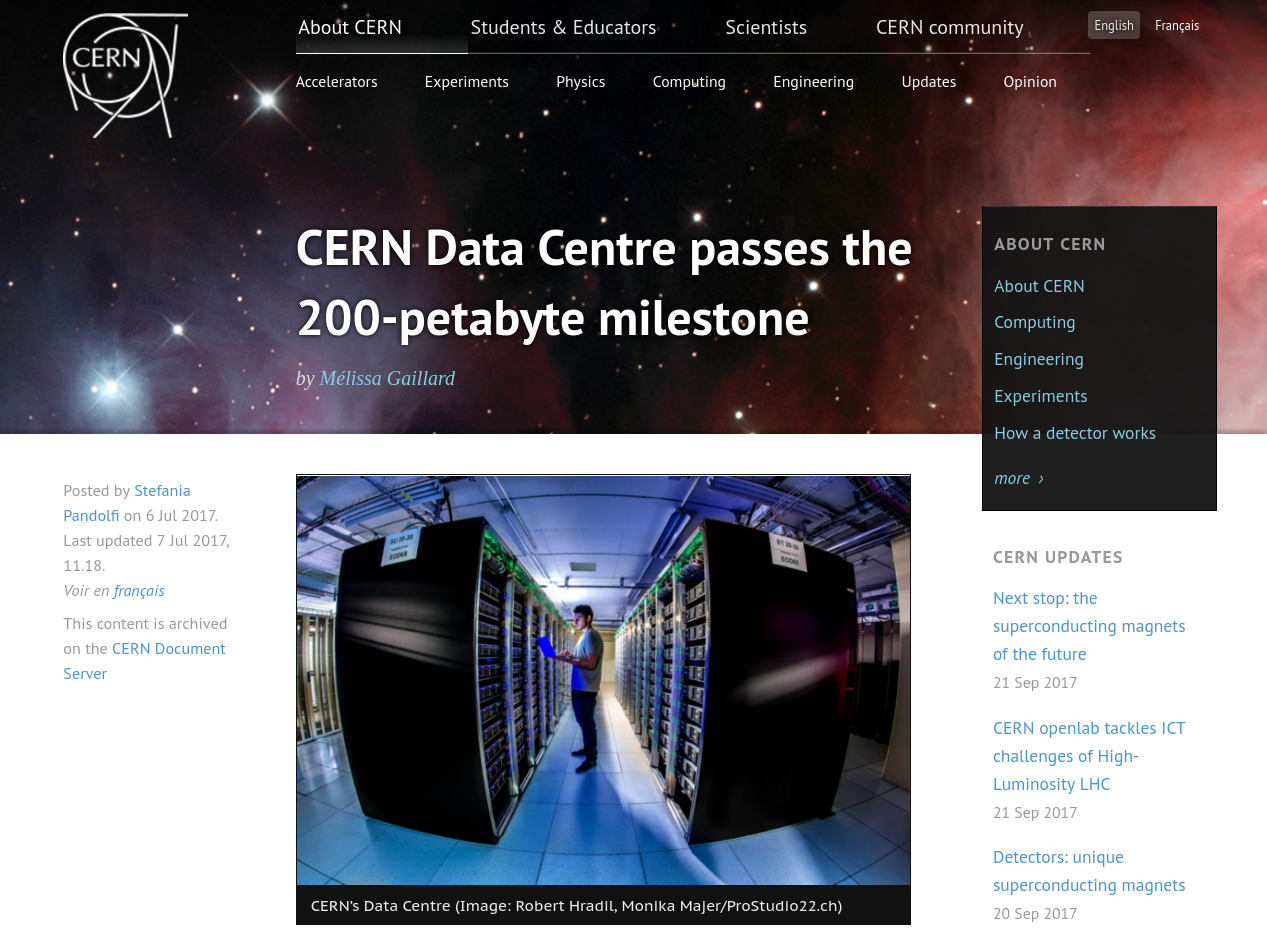
\includegraphics[width=0.73\linewidth]{cern-200pb.png}

%% \vspace{-4.8 cm}
%% \uncover<2->{\mbox{ } \hfill 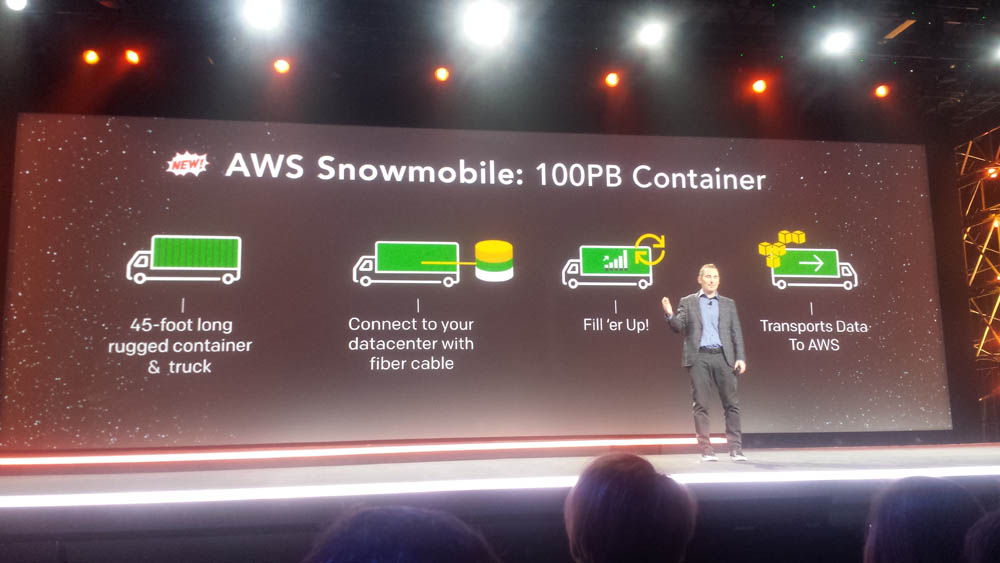
\includegraphics[width=0.7\linewidth]{aws-snowmobile.jpg}\hspace{-1 cm}}
%% \end{frame}

%% \begin{frame}{Also a much larger community}
%% \vspace{0.35 cm}
%% \textcolor{darkblue}{Rate of web searches for ``ROOT TTree'' vs.\ ``Spark DataFrame'' (Google Trends):}

%% 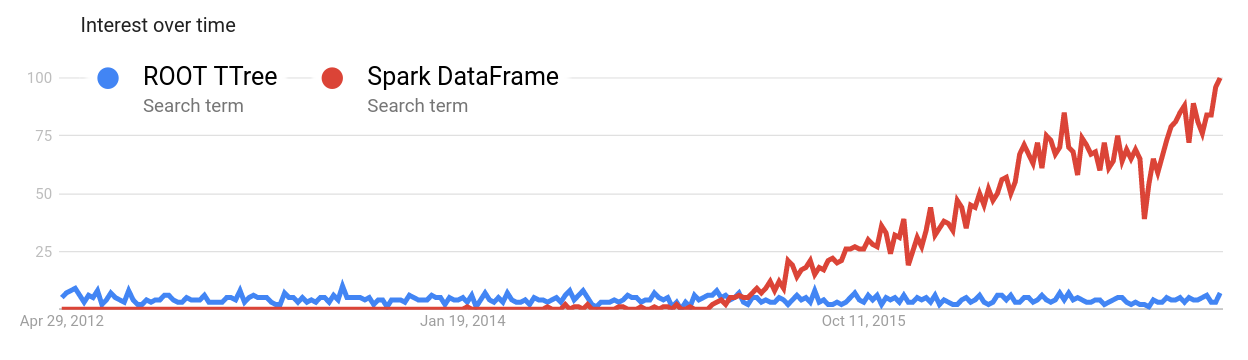
\includegraphics[width=\linewidth]{root-spark-google-trends.png}

%% \vfill
%% \begin{uncoverenv}<2->
%% \textcolor{darkblue}{Similarly for question-and-answer sites:}
%% \begin{itemize}
%% \item RootTalk: 14,399 threads in 1997--2012 (15 years)
%% \item StackOverflow questions tagged {\tt \small \#spark}: 26,155 in the 3.3 years the tag has existed. (Not counting CrossValidated, Spark Developer and User mailing lists\ldots)
%% \end{itemize}
%% \end{uncoverenv}

%% \vfill
%% \uncover<3>{\textcolor{darkorange}{\bf More users to talk to; more developers adding features/fixing bugs.}}
%% \end{frame}

%% \begin{frame}{Particle physics is a special case}
%% \vspace{-0.5 cm}
%% \begin{columns}[t]
%% \column{0.5\linewidth}
%% \begin{center}
%% \underline{\Large Particle physics}
%% \end{center}

%% \begin{itemize}
%% \item Events (modulo cosmics vetos or time-dependent calibrations) may be processed in isolation; embarrassingly parallel.

%% \item<2-> Once collected, physics datasets are immutable (possibly versioned).

%% \item<3-> Often fitting a model with a small number of parameters.

%% \end{itemize}

%% \column{0.5\linewidth}
%% \begin{center}
%% \underline{\Large Big Data}
%% \end{center}

%% \begin{itemize}
%% \item All-to-all problems are common, such as matching a customer's purchases with all other purchases to make a recommendation.

%% \item<2-> Transactions accumulate in the database during analysis.

%% \item<3-> Modeling human behavior, more interested in predictions than description, so models may have thousands of free parameters.

%% \end{itemize}

%% \end{columns}
%% \end{frame}

%% \begin{frame}{Our software is largely isolated from these developments}
%% \vspace{0.17 cm}
%% 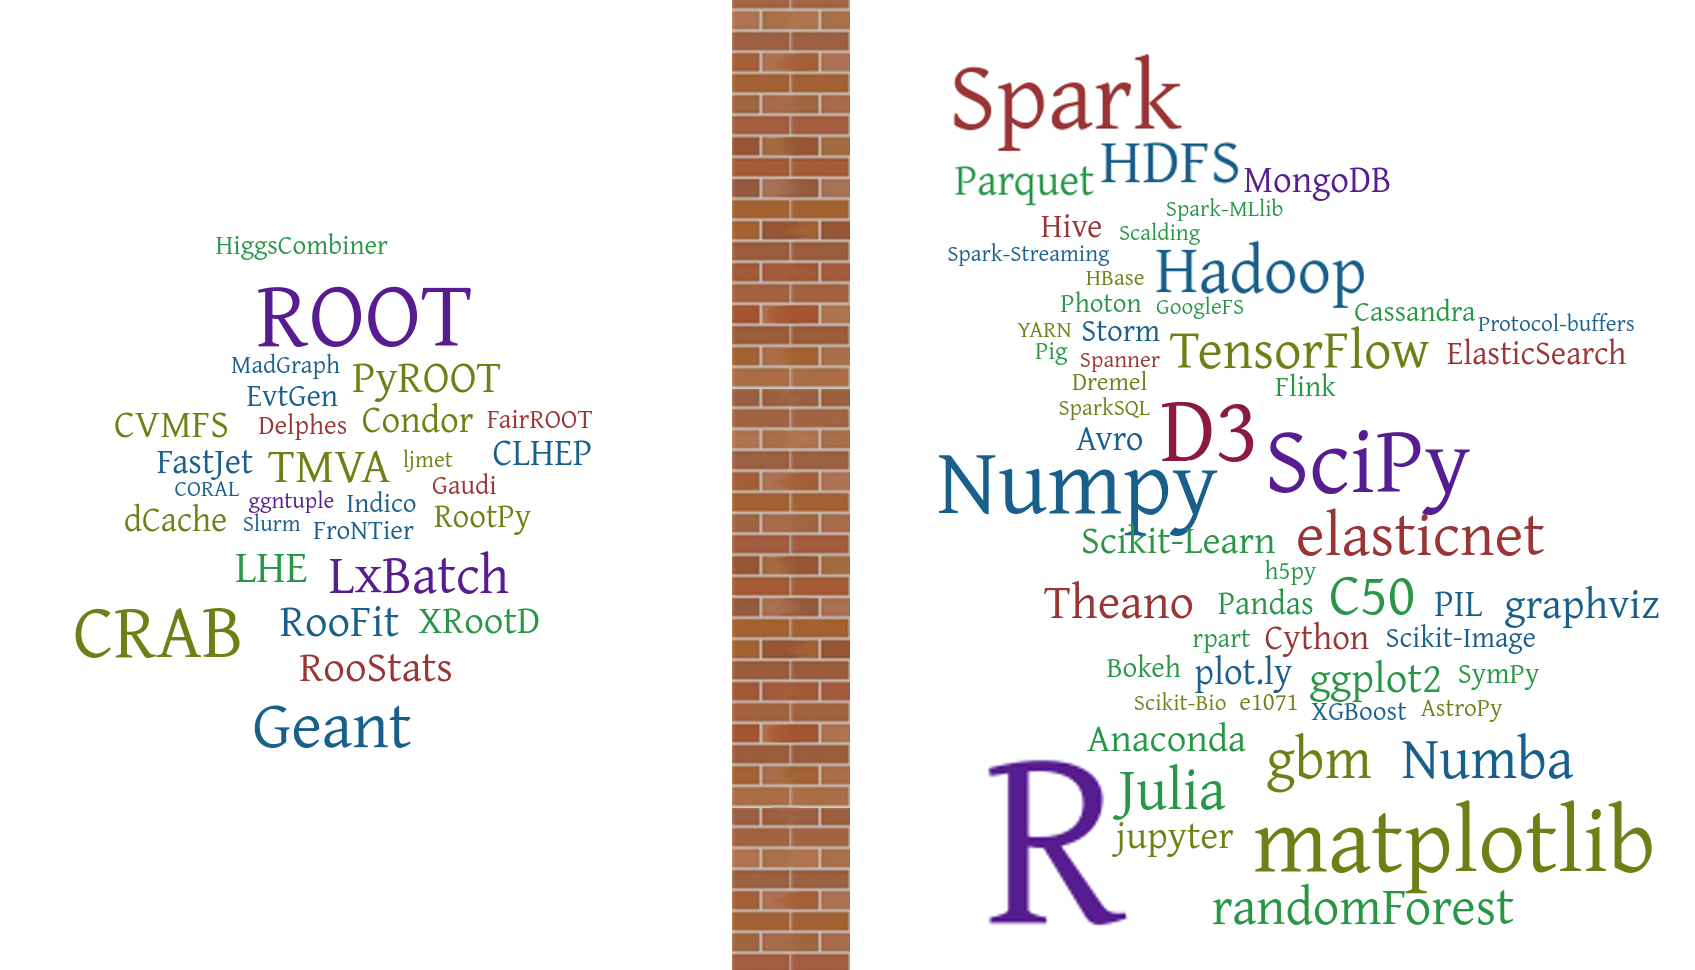
\includegraphics[width=\linewidth]{separation-2.png}
%% \end{frame}

%% \begin{frame}{But bridging the divide is worthwhile in the long run}
%% \vspace{0.5 cm}
%% \begin{center}
%% \hspace{1 cm}\only<1>{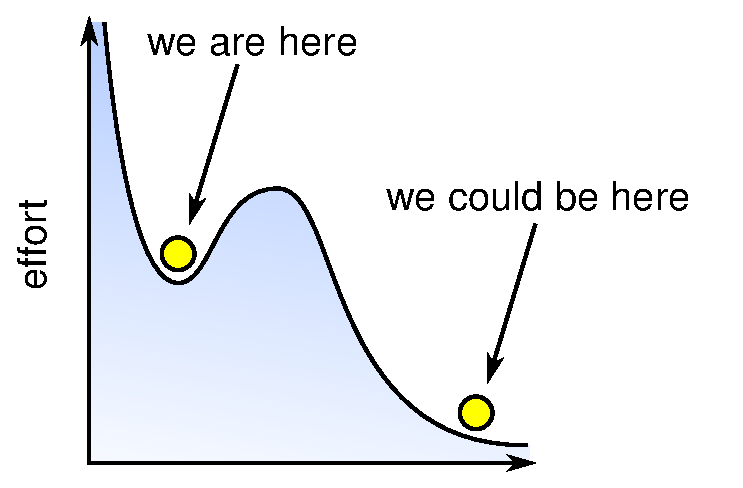
\includegraphics[width=0.65\linewidth]{effort0.pdf}}\only<2>{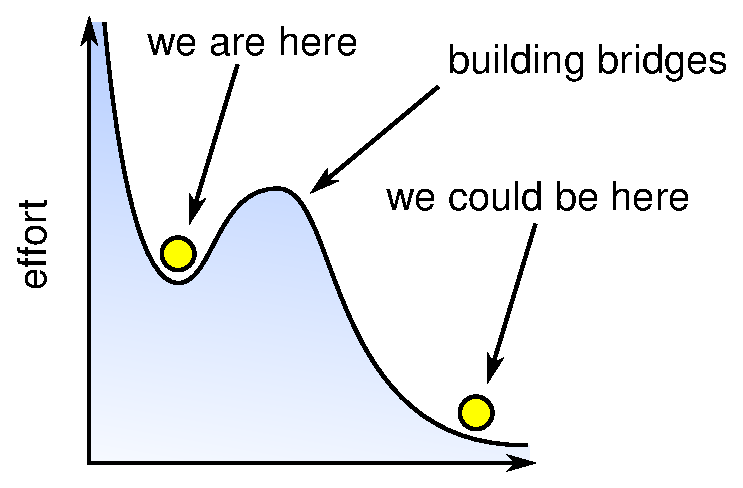
\includegraphics[width=0.65\linewidth]{effort.pdf}}
%% \end{center}
%% \end{frame}

%% \begin{frame}{Who am I?}
%% \vspace{0.5 cm}
%% \begin{columns}[t]
%% \column{0.4\linewidth}
%% \begin{columns}
%% \column{0.4\linewidth}
%% Jim Pivarski
%% \column{0.25\linewidth}
%% \hspace{-1.3 cm}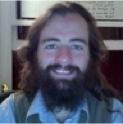
\includegraphics[width=\linewidth]{jim_pivarski.png}
%% \end{columns}

%% \begin{itemize}
%% \item 5 years CLEO (9 GeV $e^+e^-$)
%% \item 5 years CMS (7 TeV $pp$)
%% \item \only<1>{5 years Open Data Group}\only<2->{\mbox{\textcolor{darkblue}{5 years Open Data Group \hspace{0.9 cm}$\longrightarrow$\hspace{-3 cm}}}}
%% \item 2 years Project DIANA-HEP
%% \end{itemize}

%% \column{0.4\linewidth}
%% \uncover<2->{\textcolor{darkblue}{
%% hyperspectral imagery \\
%% automobile traffic \\
%% network security \\
%% Twitter sentiment \\
%% Google n-grams \\
%% DNA sequence analysis \\
%% credit card fraud detection
%% }}

%% \uncover<2->{\Large\textcolor{darkblue}{ and ``Big Data'' tools}}
%% \end{columns}

%% \vspace{0.5 cm}
%% \begin{center}
%% \uncover<3>{\large My goal within DIANA-HEP is to make it easier for physicists to use Big Data tools in their analyses, particularly for interactive, exploratory analysis.}
%% \end{center}
%% \end{frame}

\begin{frame}{}
\vspace{-0.22 cm}
\begin{center}
\only<1>{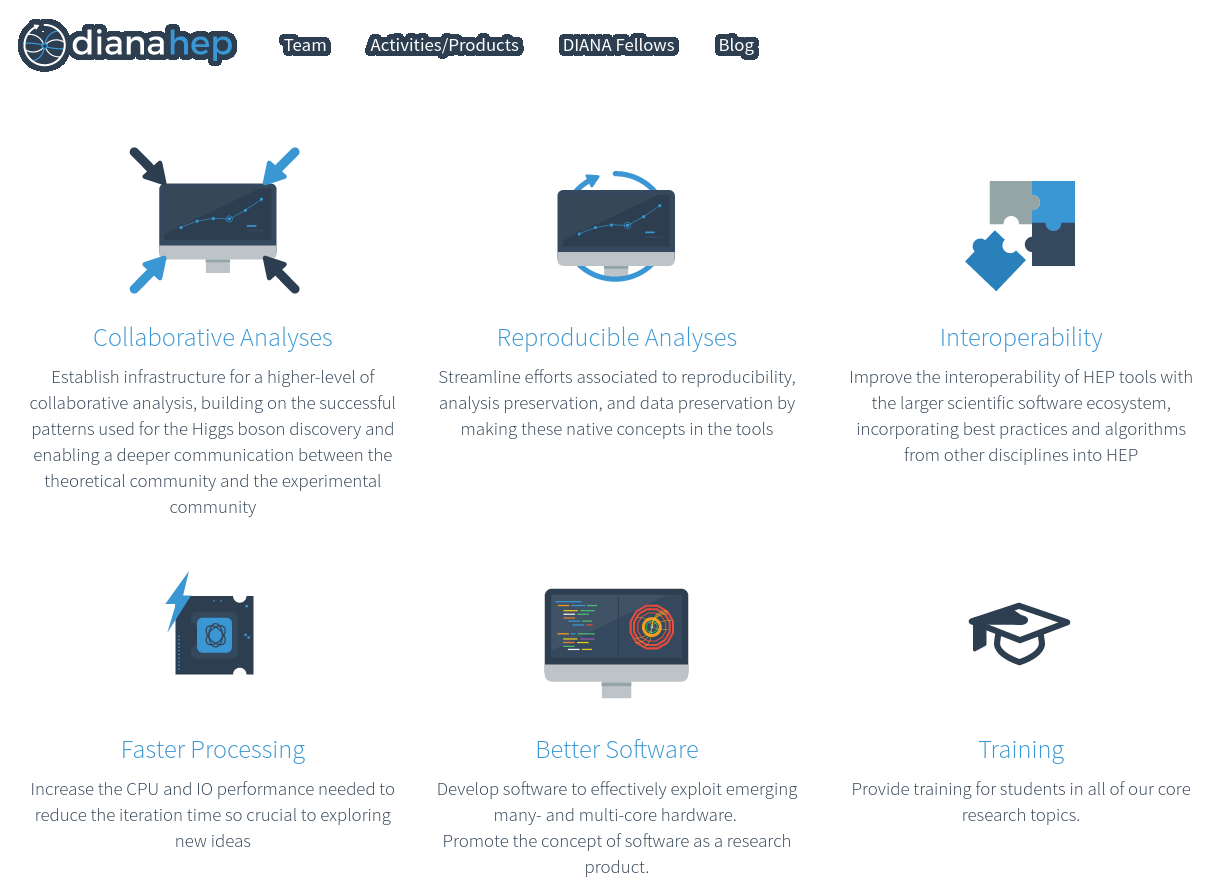
\includegraphics[width=0.88\linewidth]{diana-hep.png}}
\only<2>{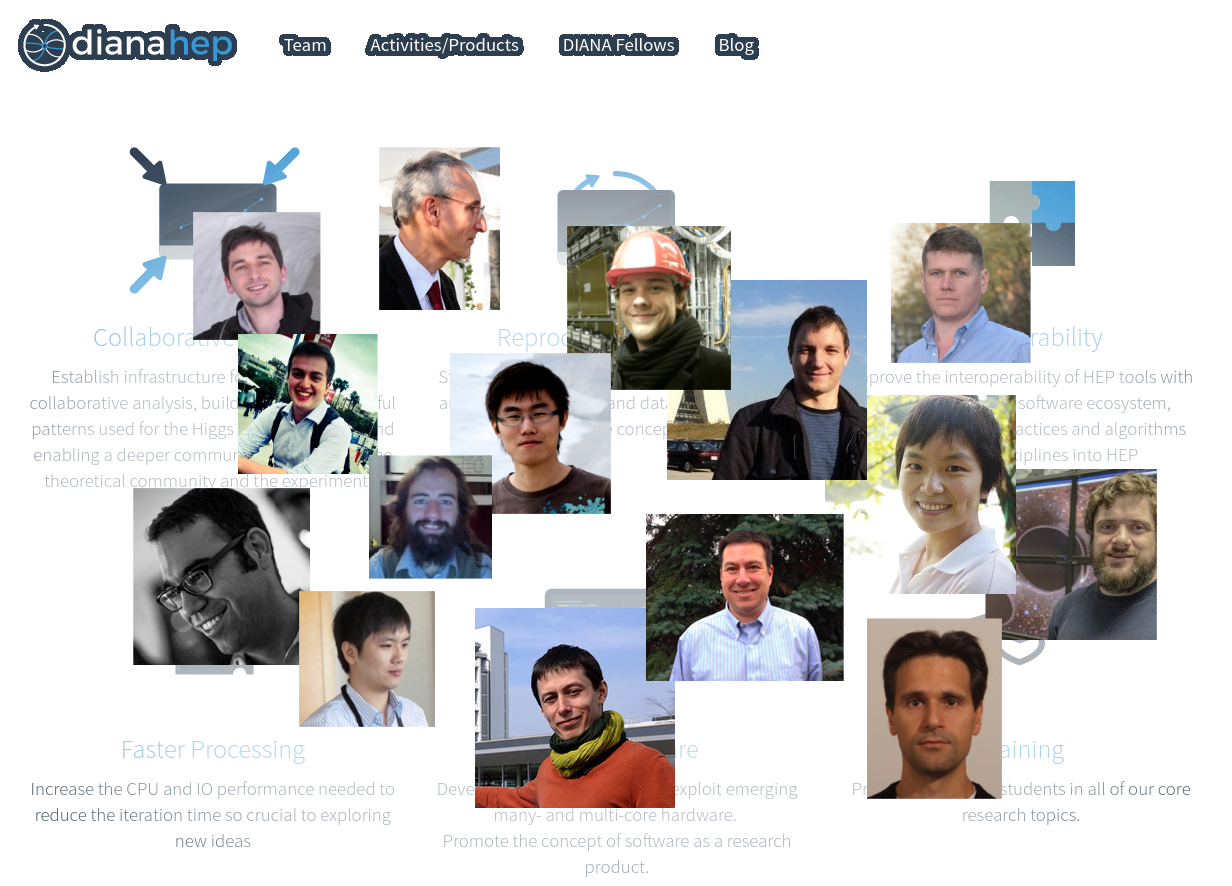
\includegraphics[width=0.88\linewidth]{diana-hep2.png}}
\end{center}
\end{frame}

%% \begin{frame}{Our problems fit into Big Data concepts}
%% \vspace{0.5 cm}
%% \begin{center}\renewcommand{\arraystretch}{2}
%% \begin{tabular}{c | c}
%% mapper (Hadoop) & skim, slim, preprocess \\
%% reducer (Hadoop) & histogramming \\
%% \begin{minipage}{0.45\linewidth}
%% \vspace{0.25 cm}
%% \begin{center}
%% data inversion

%% (e.g.\ web pages $\to$ search terms)
%% \end{center}
%% \end{minipage} & \begin{minipage}{0.45\linewidth}
%% \vspace{0.25 cm}
%% \begin{center}
%% alignment \& calibration

%% (e.g.\ track fits $\to$ detector residuals)
%% \end{center}
%% \end{minipage} \\
%% modeling & fitting \\
%% machine learning & machine learning
%% \end{tabular}
%% \end{center}

%% \vspace{0.5 cm}
%% \uncover<2->{\textcolor{darkblue}{\large So what happens if we just try to use Spark for a data analysis?}}
%% \end{frame}


\end{document}
